\chapter{Введение}\label{ch:ch1}

Данная работа посвящена верификации конкурентного кода.

Опыт показывает, что даже тщательно изученный конкурентный код может скрывать в себе ошибки:

“There is a rather large body of sad experience to indicate that a concurrent program can withstand very careful scrutiny without revealing its errors.” \autocite{Liveness}

Ошибки в конкурентном коде могут быть длинными, требующими определенного порядка действий, и в рабочей среде воспроизводиться крайне редко в силу своей недетерминированной природы. 

Поэтому критически важно иметь инструменты, которые будут помогать разработчику находить, понимать и устранять такие ошибки.

В этой главе мы сформулируем задачу верификации конкурентного кода, разберем преимущества и недостатки существующих подходов, и определим цели работы.

\section{Задача верификации}

\emph{Верификация программы} – это проверка соответствия программы предъявленным к ней требованиям \autocite{Intro}.

Нас будут интересовать программы, состоящие из нескольких потоков, взаимодействующих друг с другом через разделяемую память и синхронизирующие к ней доступ с помощью атомиков, мьютексов и условных переменных. Такие программы порождают \emph{конкурентные исполнения}, которые могут быть описаны в модели чередования потоков.

Еще точнее, мы хотим верифицировать не сами многопоточные программы (которые могут быть сколь угодно большими и сложными), а изолированные примитивы синхронизации, конкурентные структуры данных и базовые инфраструктурные компоненты. На практике весь нетривиальный конкурентный код (а вместе с ними и нетривиальные конкурентные баги) изолирован именно в подобных компонентах.

Примеры примитивов синхронизации: мьютексы, спинлоки, read-write локи, семафоры и барьеры.

Примеры конкурентных объектов: lock-free структуры данных (стек, очередь, хеш-таблица).

Примеры инфраструктурных компонентов:

\begin{itemize}

\item	Экзекьюторы для асинхронного исполнения задач (пулы потоков и декораторы над ними).

\item	Аллокаторы.
\end{itemize}

Требования формулируются в виде \emph{свойств}. В случае конкурентных объектов нас будут интересовать свойства, которые выполняются или нарушаются на отдельных исполнениях. Эти свойства можно разделить на два больших класса:

\begin{itemize}
\item	\emph{Safety (безопасность)} – никогда не случится ничего плохого.

\item	\emph{Liveness (живучесть)} – когда-нибудь случится нечто хорошее.
\end{itemize}

Это неформальные определения \autocite{Proving}, строгие формулировки приведены в \autocite{SafetyLiveness}.

Примеры safety-свойств:

\begin{itemize}
\item	\emph{Mutual exclusion} – два потока не могут одновременно находиться в критической секции.

\item	Память, отданная под узел lock-free стека, не может быть в то же время доступна для аллокации.
\end{itemize} 

Все эти свойства – \emph{инварианты} – утверждения про мгновенное состояние исполнения.

Примеры liveness-свойств:

\begin{itemize}

\item	\emph{Deadlock freedom} – если несколько потоков хотят захватить свободный мьютекс, то какой-нибудь из них в итоге войдет в критическую секцию.

\item	\emph{Starvation freedom} – все потоки когда-нибудь получат доступ к ресурсу.

\end{itemize}



\section{Подходы}

Детерминированных тестов для верификации конкурентных примитивов недостаточно: планировщик операционной системы недетерминированно переключает потоки, поэтому один и тот же код порождает несколько возможных вариантов исполнения.

Два основных подхода к верификации конкурентного кода – \emph{fault injection} и \emph{model checking}.


\subsection{Fault Injection}

Подход fault injection состоит в следующем: для примитива синхронизации или конкурентной структуры данных пишется \emph{стресс-тест} и в его исполнение недетерминированно внедряются \emph{сбои}: перепланирование (\mintinline{c++}{yield}), пауза (\mintinline{c++}{sleep}) или парковка потока. 

Также при контроле над средой исполнения сбои можно внедрять непосредственно в планировщик: рандомизировать run queue или очереди ожидания в примитивах синхронизации. Этот подход реализован в планировщике языка Go в режиме поиска гонок \autocite{Go}.

Fault injection – это механизм ускорения времени: в сравнении с обычным исполнением под управлением планировщика операционной системы мы перебираем больше нетривиальных сценариев за меньшее время.

Fault injection повышает вероятность нарушения инварианта в исполнении стресс-теста, но все же не может перебрать все возможные исполнения, а значит не может гарантировать корректность реализации тестируемого объекта.


\subsection{Model Checking}

Альтернативный подход – model checking – состоит в переборе всех возможных исполнений конкурентного кода. 

Для model checking-а пишется формальная \emph{спецификация}, которая состоит из

\begin{itemize}
\item	описания конкурентного объекта,

\item	теста для него и

\item	набора свойств.
\end{itemize}

Спецификация задает направленный \emph{граф состояний}, вершинами в котором являются все состояния исполнения, достижимые при исполнении теста, а дуги соответствуют атомарным операциям. Пути в этом графе называются \emph{траекториями}.

\emph{Model checker} по спецификации строит этот граф и проверяет на его состояниях или в общем случае путях (траекториях) заданные пользователем свойства. 

Если свойство нарушилось, то model checker предъявляет соответствующую этому нарушению траекторию: путь для safety-свойств и цикл для liveness-cвойств.

У fault injection-а и model checking-а схожие цели – исследовать граф состояний теста. Но, в отличие от fault injection-а, который перебирает отдельные траектории в графе состояний, model checking анализирует \emph{все} исполнения теста.

%\pagebreak

\subsection{+Cal / TLC}

Интерес индустрии к model checking-у начался после статьи “Use of Formal Methods at Amazon Web Services” \autocite{AWS}. В ней инженеры AWS рассказали про свой опыт верификации многопоточных структур данных и распределенных алгоритмов, лежащих в основе облачной инфраструктуры Amazon:
 
\begin{figure}
	\centerfloat{
		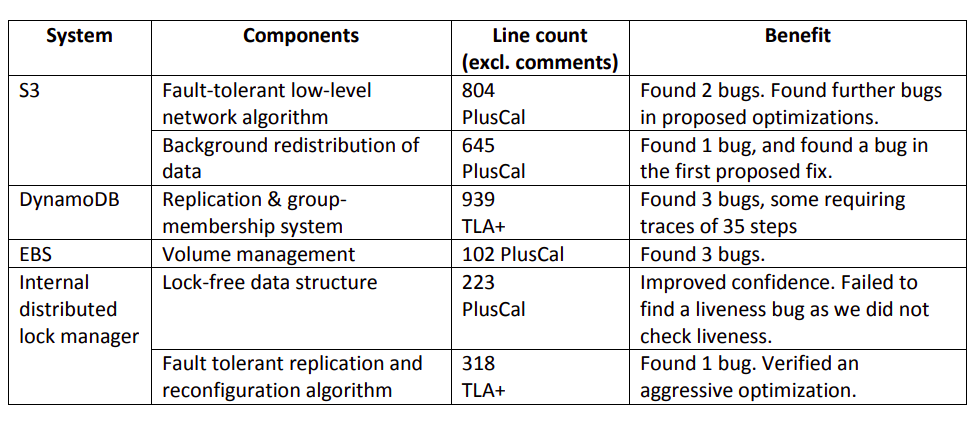
\includegraphics[scale=0.4]{aws}
	}
	\caption{Применение TLA+ / +Cal в AWS.}\label{fig:aws}
\end{figure}

Для верификации инженеры AWS выбрали языки спецификации TLA+ / +Cal и model checker TLC \autocite{Tla}. В работе мы будем говорить про +Cal, так как именно этот язык используется для спецификации многопоточного кода.

Спецификация на +Cal представляет собой псевдокод, напоминающий, в зависимости от выбранного варианта синтаксиса, код на языке C или Pascal. В качестве примера приведем фрагмент спецификации lock-free стека, написанного на C-синтаксисе языка +Cal:

\begin{figure}
\centerfloat{
\begin{tabular}{p{0.5\textwidth} p{0.5\textwidth}}
	\centering
	\vspace{0pt} 
    
    \fbox{\parbox[t][.28\textheight]{0.48\textwidth}{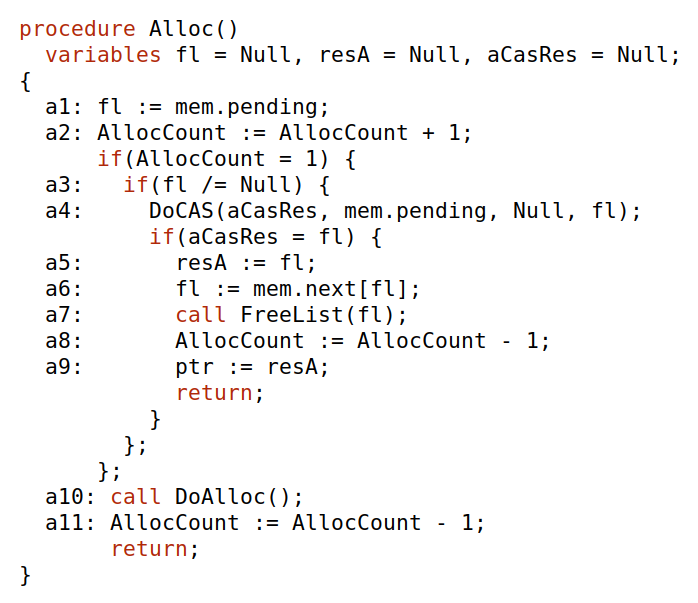
\includegraphics[width=0.48\textwidth]{specalloc}}}
    
	 &
	\vspace{0pt} 
    
    \fbox{\parbox[t][.28\textheight]{0.48\textwidth}{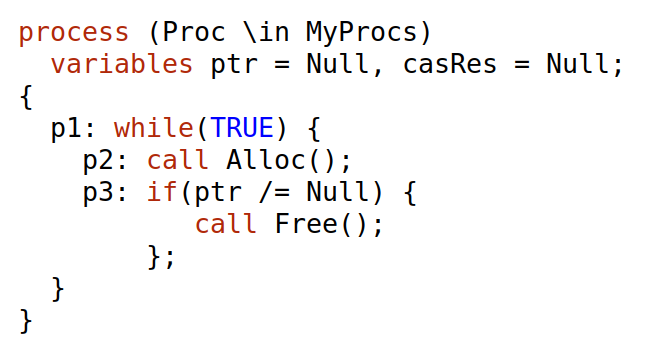
\includegraphics[width=0.35\textwidth]{spectest}}}
    
	\\
	\hfil Фрагмент алгоритма & \hfil Тест
\end{tabular}
}
\bigskip
\caption{Фрагмент спецификации lock-free стека на +Cal.}
\end{figure}



Этот псевдокод автоматически транслируется в формальный язык TLA+ и проверяется model checker-ом TLC. 

На сегодняшний день +Cal / TLC широко используется в индустрии для верификации конкурентных и распределенных алгоритмов: 

\begin{itemize}
	
\item	Спецификация конкурентных алгоритмов помогла найти баги в ядре Linux \autocite{LinuxConf} \autocite{LinuxSpec}.

\item	В Яндексе с помощью +Cal / TLC воспроизвели сценарий ABA в lock-free кеше аллокатора памяти \autocite{YaAlloc} и верифицировали исправленную версию алгоритма \autocite{YaSpec}.

\item	В Microsoft использовали +Cal для спецификации моделей согласованности распределенной базы данных CosmosDB \autocite{MsSpec}.

\item	В CockroachLabs использовали +Cal / TLC для верификации алгоритма коммита распределенных транзакций в базе данных CockroachDB \autocite{CockroachSpec}.

\end{itemize}


\subsection{Недостатки +Cal / TLC}

Хотя +Cal / TLC и являются де-факто стандартным языком спецификации / model checker-ом в индустрии, этот инструмент имеет ряд серьезных недостатков.

Самый главный и очевидный: +Cal – не язык программирования. Верифицируемый код приходится транслировать в псевдокод, а недостающие сущности – моделировать:

\begin{itemize}

\item   В +Cal нет таких сущностей как куча и указатели, их приходится заменять массивами и индексами:

\begin{figure}
	\centerfloat{
		\fbox{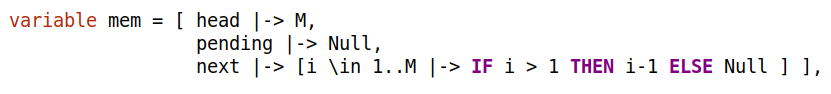
\includegraphics[scale=0.5]{calmem}}
	}
	\bigskip
	\caption{Моделирование памяти стека в +Cal.}\label{fig:calmem}
\end{figure}

\item   В +Сal нет атомарных операций. Атомарность определяется \emph{метками (labels)}: все действия в пределах одной метки являются атомарным шагом с точки зрения model checker-а. 

\end{itemize}

В результате такой трансляции можно упустить сценарий конкуренции, в котором нарушается инвариант.

Например, Лесли Лэмпорт, автор TLA+ и +Cal, в статье про проверку многопоточного алгоритма на +Cal признается, как случайно опустил метку и проверял фактически другой алгоритм: “... There is an amusing footnote to this story. After doing the checking, I noticed that I had inadvertently omitted a label from the pushRight operation, letting one atomic action access two shared variables.” \autocite{LamportPLuscal}

Траектории, найденные TLC, трудно читать. +Сal перед проверкой транслируется в спецификацию на TLA+, фактически – логический “ассемблер”, и TLC работает уже с этим “ассемблером”. В результате траектория состоит из низкоуровневого снимка стеков вызовов, служебных регистров (\mintinline{c++}{pc}) и всех переменных, в нем много нерелевантной информации. От исходного кода в траектории остаются только названия меток.

\begin{figure}
	\centerfloat{
		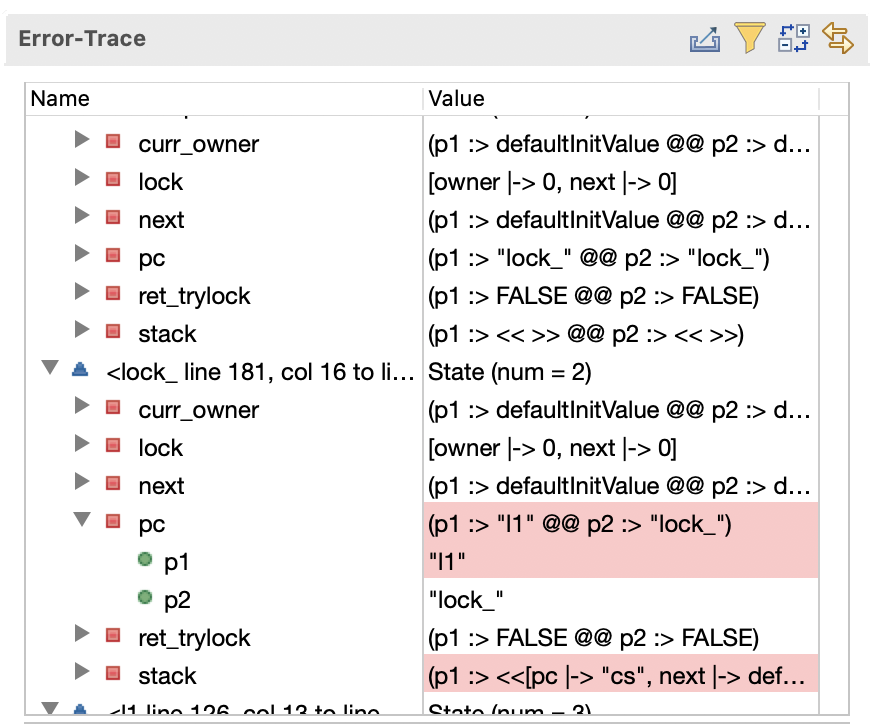
\includegraphics[scale=0.3]{caltrace}
	}
	\bigskip
	\caption{Траектория в TLA+ Toolbox.}\label{fig:caltrace}
\end{figure}

Наконец, у +Cal / TLC довольно высокий порог входа: пользователю придется изучить новый язык и разобраться с основами темпоральной логики и TLA+.

\section{Цели работы}

Для перебора всех состояний исполнения не обязательно писать на псевдокоде. Вполне можно выполнять этот перебор и над настоящим кодом. 

Цель работы – реализовать model checker, который:

\begin{itemize}
\item	{[}\emph{как +Cal / TLC}{]} Перебирает все исполнения теста.

\item	{[}\emph{как +Cal / TLC}{]} Печатает траекторию, которая приводит к нарушению инварианта. 

\item	{[}\emph{как fault injection}{]} Проверяет код на \CC, а не его модель.

\item	Показывает настоящие стектрейсы и состояния локальных переменных. 

\item	Не требует от пользователя специальных знаний в области model checking-а.
\end{itemize}

Ограничения:

\begin{itemize}
\item	Мы будем проверять не программы, а изолированные примитивы синхронизации или базовые инфраструктурные компоненты.

\item	Мы будем верифицировать только выполнение инвариантов (которые в коде тестов выражаются в виде assert-ов), и оставляем за границами работы liveness-свойства (например, livelock-и) и более сложные safety-свойства.

\item	Мы будем “разветвлять” исполнение только в точках обращения к примитивам синхронизации / атомикам. Мотивация будет приведена во второй главе работы. 

\item	Мы будем поддерживать только последовательно согласованные программы и игнорировать слабые модели памяти (\mintinline{c++}{memory_order} $\ne$ \mintinline{c++}{sec_cst}).
\end{itemize}


\section{План работы}

Во второй главе мы разберем устройство реализованного model checker-а: как перебирать исполнения многопоточного кода, как бороться с экспоненциальным ростом числа состояний, какие трудности возникают при проверке кода на \CC. 

В третьей главе мы продемонстрируем работоспособность model checker-а на двух нетривиальных примерах: lock-free аллокаторе и фреймворке экзекьюторов.

В четвертой главе мы посмотрим на инструменты, которые позволяют пользователю управлять атомарностью и отсекать ветки при переборе, выражать недетерминизм в коде теста, детализировать траекторию. 


